
% CREACIÓN DEL DOCUMENTO
\documentclass[
	spanish, % Idioma: spanish, english, etc.
	letterpaper, oneside
]{article}

% INFORMACIÓN DEL DOCUMENTO
\def\documenttitle {Mapa conceptual}
\def\documentsubtitle {Conceptos fundamentales y estructura conceptual}
\def\documentsubject {Actividad 1 - Filosofía del Derecho}

\def\documentauthor {Martín Jonathan de la Cruz}
\def\coursename {Filosofía del Derecho}
\def\coursecode {030}

\def\universityname {Universidad Abierta y a Distancia de México}
\def\universityfaculty {Licenciatura en Derecho}
\def\universitydepartment {Filosofía del Derecho}
\def\universitydepartmentimage {departamentos/UnADM}
\def\universitydepartmentimagecfg {height=1.57cm}
\def\universitylocation {Roma Norte, Ciudad de México}

% INTEGRANTES, PROFESORES Y FECHAS
\def\authortable {
	\begin{tabular}{ll}
		\textbf{Alumno:}
		& \begin{tabular}[t]{l}
			 Martín Jonathan de la Cruz \\	
		\end{tabular} \\
		Matrícula: &   ES2611202040 \\
		
		Profesor:
		& \begin{tabular}[t]{l}
			Reyna Patricia \\ Gonzales Rodríguez
		\end{tabular} \\
		% Auxiliar:
		% & \begin{tabular}[t]{l}
		% 	Auxiliar 1
		% \end{tabular} \\
		% Ayudantes:
		% & \begin{tabular}[t]{l}
		% 	Ayudante 1 \\
		% 	Ayudante 2
		% \end{tabular} \\
		% \multicolumn{2}{l}{Ayudante de laboratorio: Ayudante 1} \\
		& \\
		\multicolumn{2}{l}{Fecha de realización: \today} \\
		% \multicolumn{2}{l}{Fecha de entrega: \today} \\
		\multicolumn{2}{l}{\universitylocation}
	\end{tabular}
}

% IMPORTACIÓN DEL TEMPLATE
\input{template}
\setcitestyle{authoryear,open={(},close={)}}

% FUENTE HELVETICA / SANS-SERIF
\usepackage[T1]{fontenc}
\usepackage{helvet}
\renewcommand{\familydefault}{\sfdefault}

% MARCA DE AGUA / PRODUCTO VISUAL
\usepackage{tikz}
\usepackage{pdflscape}

% ==============================================================================
% MARCA DE AGUA EN PORTADA
% - Se aplica solo a la portada porque usa \AddToShipoutPictureBG*.
% - Para apagarla en alguna actividad: \def\coverwatermarkenabled {false}
% - Usar opacidad baja para que no compita con titulo, datos ni logotipo.
% ==============================================================================
\def\coverwatermarkenabled {true}
\def\coverwatermarkimage {img/departamentos/UnADM.pdf}
\def\coverwatermarkopacity {0.16}
\def\coverwatermarkwidth {0.72\paperwidth}
\def\coverwatermarkxshift {0cm}
\def\coverwatermarkyshift {-0.35cm}

\newcommand{\insertcoverwatermark}{%
	\ifthenelse{\equal{\coverwatermarkenabled}{true}}{%
		\AddToShipoutPictureBG*{%
			\begin{tikzpicture}[remember picture,overlay]
				\node[
					opacity=\coverwatermarkopacity,
					inner sep=0pt,
					xshift=\coverwatermarkxshift,
					yshift=\coverwatermarkyshift
				] at (current page.center) {%
					\includegraphics[width=\coverwatermarkwidth]{\coverwatermarkimage}%
				};
			\end{tikzpicture}%
		}%
	}{}%
}

% INICIO DE PÁGINAS
\begin{document}

% PORTADA
\insertcoverwatermark
\templatePortrait

% CONFIGURACIÓN DE PÁGINA Y ENCABEZADOS
\templatePagecfg

% RESUMEN O ABSTRACT
\begin{abstractd}
	\textbf{Objetivo:} Comprender los fundamentos conceptuales y las principales corrientes filosóficas de la Filosofía del Derecho, identificando y analizando las teorías de importantes pensadores y su influencia en la estructura y evolución del sistema legal, con el fin de desarrollar una visión crítica y reflexiva sobre el derecho en la sociedad contemporánea.
	\newline

	\textbf{Propósito:} Identificar los conceptos básicos de la Filosofía del Derecho para reconocer la importancia de su aplicación en el sistema jurídico.


\end{abstractd}

% TABLA DE CONTENIDOS - ÍNDICE
\templateIndex

% CONFIGURACIONES FINALES
\templateFinalcfg

% ======================= MAPA CONCEPTUAL EN PÁGINA LANDSCAPE =======================
% Página sin encabezados ni pies

\newpage
\thispagestyle{empty}
\begin{landscape}

\begin{figure}[h!]
\centering
\vspace*{-1.5cm}
\resizebox{0.96\linewidth}{!}{%
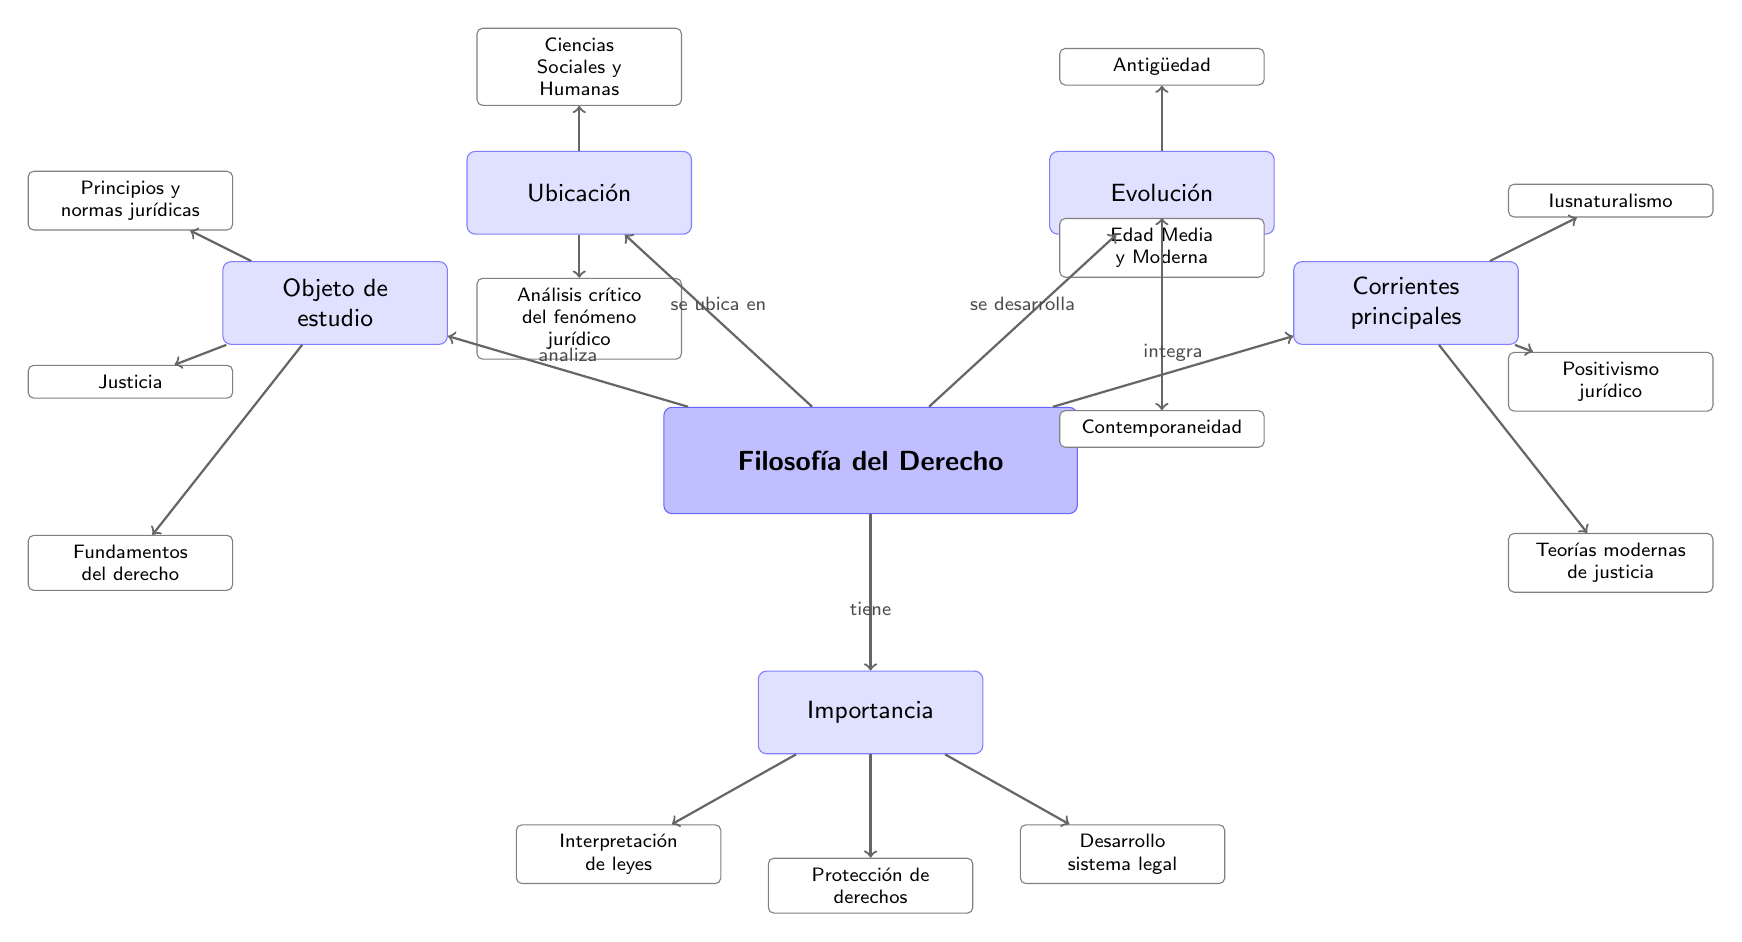
\begin{tikzpicture}[
	concept/.style={
		rectangle,
		rounded corners=3pt,
		draw=black!70,
		fill=gray!8,
		align=center,
		text width=3.0cm,
		minimum height=1.05cm,
		inner sep=5pt,
		font=\sffamily\small
	},
	root/.style={
		concept,
		fill=blue!25,
		draw=blue!60,
		text width=4.9cm,
		minimum height=1.35cm,
		font=\bfseries\sffamily\normalsize
	},
	branch/.style={
		concept,
		fill=blue!12,
		draw=blue!50,
		text width=2.5cm
	},
	subbranch/.style={
		rectangle,
		rounded corners=2pt,
		draw=black!50,
		fill=white,
		align=center,
		text width=2.35cm,
		inner sep=3.5pt,
		font=\sffamily\scriptsize
	},
	edge/.style={->,thick,black!60},
	label/.style={font=\sffamily\scriptsize,black!70}
]

% Nodo central
\node[root] (root) at (0,0) {\textbf{Filosofía del Derecho}};

% Rama 1: Objeto de estudio
\node[branch] (obj) at (-6.8,2.0) {Objeto de\\estudio};
\node[subbranch] (obj1) at (-9.4,3.3) {Principios y\\normas jurídicas};
\node[subbranch] (obj2) at (-9.4,1.0) {Justicia};
\node[subbranch] (obj3) at (-9.4,-1.3) {Fundamentos\\del derecho};

% Rama 2: Ubicación
\node[branch] (ubic) at (-3.7,3.4) {Ubicación};
\node[subbranch] (ubic1) at (-3.7,5.0) {Ciencias\\Sociales y\\Humanas};
\node[subbranch] (ubic2) at (-3.7,1.8) {Análisis crítico\\del fenómeno\\jurídico};

% Rama 3: Evolución
\node[branch] (evol) at (3.7,3.4) {Evolución};
\node[subbranch] (evol1) at (3.7,5.0) {Antigüedad};
\node[subbranch] (evol2) at (3.7,2.7) {Edad Media\\y Moderna};
\node[subbranch] (evol3) at (3.7,0.4) {Contemporaneidad};

% Rama 4: Corrientes
\node[branch] (corr) at (6.8,2.0) {Corrientes\\principales};
\node[subbranch] (corr1) at (9.4,3.3) {Iusnaturalismo};
\node[subbranch] (corr2) at (9.4,1.0) {Positivismo\\jurídico};
\node[subbranch] (corr3) at (9.4,-1.3) {Teorías modernas\\de justicia};

% Rama 5: Importancia
\node[branch] (imp) at (0,-3.2) {Importancia};
\node[subbranch] (imp1) at (-3.2,-5.0) {Interpretación\\de leyes};
\node[subbranch] (imp2) at (0,-5.4) {Protección de\\derechos};
\node[subbranch] (imp3) at (3.2,-5.0) {Desarrollo\\sistema legal};

% Conexiones rama 1
\draw[edge] (root) -- node[label,above]{analiza} (obj);
\draw[edge] (obj) -- (obj1);
\draw[edge] (obj) -- (obj2);
\draw[edge] (obj) -- (obj3);

% Conexiones rama 2
\draw[edge] (root) -- node[label,above]{se ubica en} (ubic);
\draw[edge] (ubic) -- (ubic1);
\draw[edge] (ubic) -- (ubic2);

% Conexiones rama 3
\draw[edge] (root) -- node[label,above]{se desarrolla} (evol);
\draw[edge] (evol) -- (evol1);
\draw[edge] (evol) -- (evol2);
\draw[edge] (evol) -- (evol3);

% Conexiones rama 4
\draw[edge] (root) -- node[label,above]{integra} (corr);
\draw[edge] (corr) -- (corr1);
\draw[edge] (corr) -- (corr2);
\draw[edge] (corr) -- (corr3);

% Conexiones rama 5
\draw[edge] (root) -- node[label,below]{tiene} (imp);
\draw[edge] (imp) -- (imp1);
\draw[edge] (imp) -- (imp2);
\draw[edge] (imp) -- (imp3);

\end{tikzpicture}
}%
\caption{Mapa Conceptual de la Filosofía del Derecho - Semana 2}
\label{fig:mapa-conceptual-filosofia}
\end{figure}

\vspace{-0.5cm}
\end{landscape}

% ======================= INICIO DEL DOCUMENTO =======================

\section{Introducción}

\begin{flushleft}
La Filosofía del Derecho es una disciplina fundamental que se encarga de analizar los principios, fundamentos y estructuras conceptuales del derecho. A través de esta actividad, se busca comprender los elementos esenciales que configuran el pensamiento jurídico, desde sus orígenes hasta las corrientes contemporáneas.

El presente trabajo tiene como objetivo identificar y mapear conceptualmente los aspectos clave de la Filosofía del Derecho, tales como su objeto de estudio, ubicación dentro del sistema de ciencias, evolución histórica, principales corrientes de pensamiento e importancia en la práctica jurídica actual.

Para lograr esto, se realizará una revisión exhaustiva de la bibliografía propuesta, se identificarán los conceptos fundamentales y se elaborará un mapa conceptual que sintetice estas ideas de manera clara y visual. Esta actividad permitirá desarrollar una comprensión crítica sobre la influencia de la filosofía jurídica en la estructura y evolución del sistema legal.
\end{flushleft}

\section{Conceptos Fundamentales de la Filosofía del Derecho}

La lectura del material permite identificar cinco conceptos clave que ordenan la disciplina. Su \textbf{objeto de estudio} son los principios, normas y sistemas jurídicos, junto con los fundamentos de la justicia y el derecho natural \cite{finnisEstudiosTeoriaDerecho2017,lovonManualPracticoFilosofia2020}. En cuanto a su \textbf{ubicación}, se trata de una disciplina de las ciencias sociales y humanas que analiza críticamente el fenómeno jurídico \cite{ruizrodriguezFilosofiaDerecho2009}.

Su \textbf{evolución} recorre desde la antigüedad hasta la contemporaneidad, con énfasis en las teorías iusnaturalistas y positivistas. Las \textbf{corrientes} principales comprenden el iusnaturalismo, el positivismo jurídico y las teorías modernas de justicia \cite{finnisEstudiosTeoriaDerecho2017,ruizrodriguezFilosofiaDerecho2009,lovonManualPracticoFilosofia2020}. Finalmente, su \textbf{importancia} se aprecia en la interpretación y evolución del derecho y en los sistemas de protección de derechos fundamentales \cite{cpeum2026,LeyAmparoReglamentaria}.

\subsection{Fundamentos Teóricos Identificados}

Según la bibliografía analizada:

\paragraph{Derecho Natural y Justicia}
El enfoque de Finnis en los estudios de teoría del derecho natural es fundamental para comprender cómo los principios universales de justicia y equidad configuran los sistemas legales \cite{finnisEstudiosTeoriaDerecho2017}. Esta perspectiva contrasta con el positivismo jurídico pero ambas corrientes son esenciales para la comprensión integral de la filosofía del derecho.

\paragraph{Fundamentos Prácticos}
Lovón enfatiza la importancia de los fundamentos prácticos del derecho y la justicia, vinculando la teoría filosófica con la aplicación real en sistemas legales \cite{lovonManualPracticoFilosofia2020}. Esto se refleja en los textos legales mexicanos como la Constitución Política, la Ley de Amparo, la Ley General de Víctimas y la Ley de Acceso de las Mujeres a una Vida Libre de Violencia \cite{cpeum2026,LeyAmparoReglamentaria,LeyGeneralVictimas,franzoniacevedoLeyGeneralAcceso2017}.

\paragraph{Principios Fundamentales}
Los textos legales mexicanos revelan principios clave que operan de forma encadenada: la legalidad y la constitucionalidad fijan el marco de validez; la justicia y la equidad orientan su contenido; la protección de derechos fundamentales define el bien tutelado; el acceso a la justicia habilita la vía para exigirlo; y la reparación de víctimas cierra el ciclo cuando el daño ya ocurrió. \textbf{Desde mi perspectiva}, esa secuencia muestra que ningún principio basta por sí solo: sin acceso a la justicia, la protección queda en enunciado.
\section{Estructura Conceptual: Análisis de Elementos Fundamentales}

\subsection{Objeto de Estudio}

Según la bibliografía analizada, el objeto de estudio de la Filosofía del Derecho incluye:

\begin{enumerate}
	\item \textbf{Principios Jurídicos}: Son los principios que rigen la actividad jurídica y que sirven como base para la interpretación y aplicación de las normas legales. Estos principios pueden incluir la legalidad, la justicia, la equidad, entre otros \cite{finnisEstudiosTeoriaDerecho2017,lovonManualPracticoFilosofia2020}.
	\item \textbf{Normas y Sistemas Legales}: Son las reglas y principios que rigen el comportamiento humano en el ámbito jurídico, establecidas por autoridades competentes y que tienen efecto vinculante \cite{rojas-gonzalezFilosofiaDerecho2018,lastraConceptosJuridicosFundamentales}.
	\item \textbf{Justicia}: Es el principio moral y legal que busca la equidad en la distribución de bienes y servicios dentro de una sociedad \cite{finnisEstudiosTeoriaDerecho2017,lovonManualPracticoFilosofia2020}.
	\item \textbf{Fundamentos del Derecho}: Son los principios básicos que sustentan la existencia y funcionamiento del sistema jurídico \cite{ruizrodriguezFilosofiaDerecho2009,lastraConceptosJuridicosFundamentales}.
\end{enumerate}

\subsection{Corrientes Principales}

Tres corrientes organizan el estudio filosófico del derecho. El \textbf{Derecho Natural} sostiene que existen principios universales de justicia inherentes a la naturaleza humana, que los sistemas legales deben respetar \cite{finnisEstudiosTeoriaDerecho2017}. \textbf{En cambio}, el \textbf{Positivismo Jurídico} entiende el derecho como un conjunto de normas creadas por la autoridad competente, sin vínculo necesario con principios morales \cite{ruizrodriguezFilosofiaDerecho2009}.

\textbf{Por consiguiente}, las \textbf{Teorías Modernas de Justicia} surgen como intento de integrar ambas posiciones, al enfatizar la equidad y la protección de derechos fundamentales en el sistema jurídico contemporáneo \cite{lovonManualPracticoFilosofia2020,lastraConceptosJuridicosFundamentales}. \textbf{A mi juicio}, esa integración es la posición más defendible: reconoce que la norma requiere forma institucional sin renunciar al examen sobre su contenido.

\subsection{Elementos Fundamentales}

Cuatro elementos sostienen el análisis. Los \textbf{Derechos Fundamentales} son las prerrogativas básicas e inalienables de toda persona, que el sistema jurídico debe proteger \cite{cpeum2026,LeyAmparoReglamentaria}. Los \textbf{Principios Éticos} operan como los valores morales que guían la conducta humana e influyen en la creación y aplicación de las normas \cite{finnisEstudiosTeoriaDerecho2017,lovonManualPracticoFilosofia2020}.

\textbf{Además}, el \textbf{Ordenamiento Legal} reúne las normas jurídicas que regulan la convivencia social y que aplican las autoridades competentes \cite{rojas-gonzalezFilosofiaDerecho2018}, mientras que las \textbf{Instituciones Jurídicas} son las estructuras que hacen posible administrar justicia \cite{lastraConceptosJuridicosFundamentales}. \textbf{Es decir}, los dos primeros elementos aportan el contenido y los dos últimos la forma que lo vuelve operativo.

\subsection{Aplicaciones Prácticas}

La disciplina se proyecta en tres aplicaciones prácticas. El \textbf{Sistema Constitucional} mexicano fija el marco de derechos y obligaciones de ciudadanos y autoridades, y sirve de base para interpretar y aplicar las normas \cite{cpeum2026}. Los \textbf{Mecanismos de Protección} son los instrumentos que permiten defender los derechos fundamentales frente a violaciones de autoridades o particulares \cite{LeyAmparoReglamentaria,LeyGeneralVictimas,franzoniacevedoLeyGeneralAcceso2017}. \textbf{Por último}, la \textbf{Solución de Controversias} agrupa métodos alternativos como la mediación o el arbitraje, que resuelven conflictos sin proceso judicial formal \cite{lastraConceptosJuridicosFundamentales}.

\section{Conclusión}

Con base en el análisis de la bibliografía especializada en Filosofía del Derecho, se ha logrado identificar y sintetizar los conceptos fundamentales que configuran esta disciplina como un campo esencial de estudio en las ciencias sociales y humanas.

\paragraph{Hallazgos principales y postura propia:}

El análisis realizado me lleva a sostener que la Filosofía del Derecho es una disciplina integral: no se limita al análisis teórico, sino que articula las perspectivas iusnaturalista y positivista mediante un diálogo crítico que amplía la comprensión del fenómeno jurídico \cite{finnisEstudiosTeoriaDerecho2017,ruizrodriguezFilosofiaDerecho2009,lovonManualPracticoFilosofia2020}. Sin embargo, esta articulación no elimina la importancia del contexto, pues los principios de justicia y derecho natural adquieren manifestaciones concretas según las condiciones históricas, sociales y culturales; el marco jurídico mexicano permite observar esa relación \cite{cpeum2026,LeyAmparoReglamentaria,LeyGeneralVictimas}.

Por ello, considero que el conocimiento filosófico-jurídico tiene una función práctica: orienta la interpretación del derecho y permite valorar la protección de los derechos fundamentales y los mecanismos de justicia alternativa, no solo describir las normas vigentes \cite{lastraConceptosJuridicosFundamentales}. En consecuencia, la justicia funciona como criterio articulador de principios, normas y prácticas, y el mapa conceptual resulta pertinente porque hace visible esa relación entre fundamentos teóricos, ordenamiento jurídico y aplicación social.

\paragraph{Relevancia contemporánea y postura propia:}

Considero que la legislación mexicana sobre protección de víctimas, derechos de las mujeres y mecanismos alternativos de solución de controversias ofrece un referente concreto para examinar cómo los principios de justicia, igualdad y acceso a la justicia orientan la respuesta jurídica ante problemas sociales contemporáneos \cite{LeyGeneralVictimas,franzoniacevedoLeyGeneralAcceso2017,lastraConceptosJuridicosFundamentales}. Desde esta perspectiva, la Filosofía del Derecho no sustituye el análisis de las normas vigentes, sino que aporta criterios para valorar críticamente su finalidad y sus efectos.

En conclusión, la Filosofía del Derecho constituye un campo interdisciplinario, crítico y reflexivo que proporciona herramientas conceptuales para comprender y evaluar los sistemas de justicia desde la exigencia de mayor equidad y protección de los derechos fundamentales.\footnote{En la elaboración de este trabajo se utilizaron herramientas de inteligencia artificial como apoyo para la organización y revisión del texto, conforme a los Lineamientos para el uso ético y responsable de la Inteligencia Artificial en el ámbito académico de la UnADM. El análisis, la selección de fuentes y la postura sostenida son de mi autoría.}

\clearpage

\bibliography{filosofia-del-derecho}

% FIN DEL DOCUMENTO
\end{document}
